\section{Theory}
\subsection{Conservation properties of FVM}
We will begin by going into detail about the conservation properties of FVM. When we have a large global volume and split it into several smaller local volumes we introduce new common surfaces between the local volumes. This have an effect when we apply the Gauss-Divergence theorem to go from volume integrals to surface integrals as we now integrate over the surfaces. To illustrate this we can define some vector function $\mathbf{f}(\mathbf{u})$ and integrate the divergence of this function over some fixed volume \textit{V} giving us:
\begin{equation*}
	\int_V \nabla\cdot\mathbf{f}(\mathbf{u})dV
\end{equation*}
Converting this to a surface integral we apply Gauss-Divergence theorem giving us:
\begin{equation*}
	\int_S \mathbf{f}(\mathbf{u})\cdot\mathbf{n}dS
\end{equation*}
Where \textbf{n} is the outwards unit normal. However, as discussed and illustrated in \autoref{conservation} by splitting the global volume we have introduced a new surface. Looking at  \autoref{conservation} we have $V_a$ and $V_b$ share the common surface $S_c$, the boundary of $V_a$ is $S_a \cup S_c$ and the boundary of $V_b$ is $S_b \cup S_c$. We also note $V = V_a \cup V_b$ and $S = S_a \cup S_b$. We can thus integrate over the local volumes and get:
\begin{align*}
	\int_{V_a\cup V_b}\nabla\cdot\mathbf{f}(\mathbf{u})dV &= \int_{S_a} \mathbf{f}(\mathbf{u})\cdot\mathbf{n_a}dS + \int_{S_c} \mathbf{f}(\mathbf{u})\cdot\mathbf{n_c}dS\\ 
	&+\int_{S_b} \mathbf{f}(\mathbf{u})\cdot\mathbf{n_b}dS + \int_{S_c} \mathbf{f}(\mathbf{u})\cdot(-\mathbf{n_c})dS
\end{align*}
We here see the integrals over the common surface cancels out giving us:
\begin{equation*}
	\int_{V_a\cup V_b}\nabla\cdot\mathbf{f}(\mathbf{u})dV = \int_{S_a\cup S_b} \mathbf{f}(\mathbf{u})\cdot\mathbf{n}dS
\end{equation*}
Which is equivalent to:
\begin{equation*}
	\int_V\nabla\cdot\mathbf{f}(\mathbf{u})dV = \int_S \mathbf{f}(\mathbf{u})\cdot\mathbf{n}dS
\end{equation*}
This means conservation is guaranteed on both a local and a global scale.

\begin{figure}
	\centering
	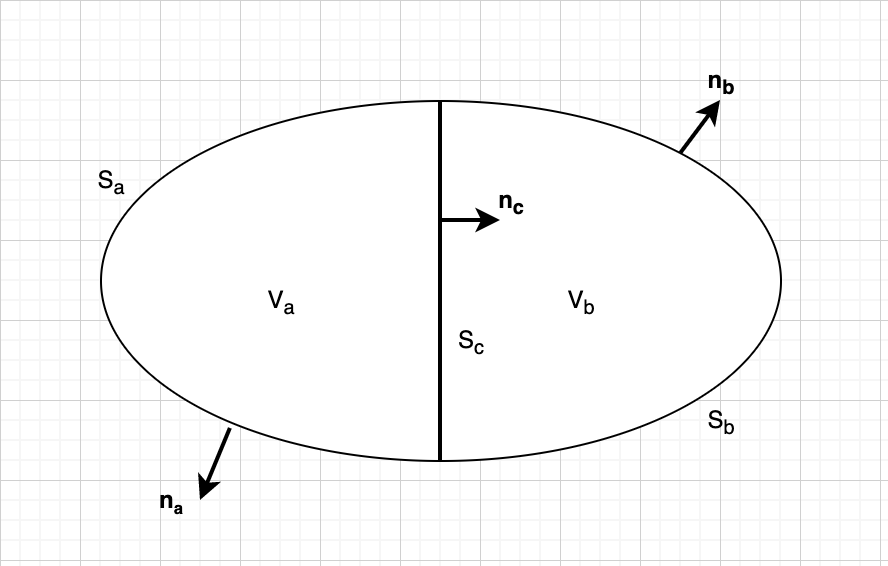
\includegraphics[width=0.7\linewidth]{Materials/Conservation}
	\caption{Illustration of a global volume getting split introducing a new common surface.}
	\label{conservation}
\end{figure}

\subsection{Control volumes}
An integral part of FVM is the control volumes. Control volumes are introduced as part of our discretization to simplify our problem such that we look at a local subproblem which is easier to solve. Control volumes can be of any shape as long as we have the geometric information of them, e.g. cell centers, surface centers, neighbouring cells, surface connectivity etc. For this week's assignment we will construct a regular triangle mesh. In this mesh we will define the control volumes 'around' vertices of the mesh. That is, in the interior of the mesh we will construct octagons and squares going between the centers of our triangle mesh. At the boundaries of our mesh we will create polygons. This can be seen in \autoref{controlvolume}. Although there are no formal requirements on the shape of the control volumes we need the edges of the control volumes to be perpendicular to the grid lines in our mesh, otherwise the outwards unit normal of the control volume surface will point in a different direction than the line segments connecting our vertices and we will introduce errors in our later approximations. Because of this we need to tailor the shape of our control volumes such that they match with our choice of mesh.

\subsection{FVM applied to Magnetostatic problem}
We can now apply FVM to our problem in this week's notebook, namely the Magnetostatic problem which has the PDE $\nabla \cdot \nabla \phi(\mathbf{x}) = \nabla \cdot \mathbf{M}(\mathbf{x})$. The first step of FVM is to decide on a mesh and control volume layout. As we are dealing with a 2D problem in the notebook we will use a regular triangle mesh. For control volumes we will use the centers in the triangles to draw octagons and squares between interior nodes, and simple lines to the boundary. This is illustrated in \autoref{controlvolume} where black lines is our mesh and red lines constitute our control volumes. The next step is to convert our PDE to a volume integral and then to a surface integral using the \textit{Gauss-Divergence theorem}.
\begin{align*}
	\nabla \cdot \nabla \phi(\mathbf{x}) &= \nabla \cdot \mathbf{M}(\mathbf{x})\\
	\int_V\nabla \cdot \nabla \phi(\mathbf{x})dV &= \int_V \nabla \cdot \mathbf{M}(\mathbf{x})dV\\
	\int_S\nabla \phi(\mathbf{x})\cdot \mathbf{n}dS &= \int_S \mathbf{M}(\mathbf{x})\cdot \mathbf{n}dS
\end{align*}
Where $\mathbf{n}$ is the outward unit normal. These surface integrals means we need to integrate over the edges of our control volumes. We can now exploit that the edges are piecewise continuous, making our integrals \textit{piecewise continuous integrals}. 
\begin{equation*}
	\sum_e\int_{S_e}\nabla \phi(\mathbf{x})\cdot \mathbf{n_e}dS = \sum_e\int_{S_e} \mathbf{M}(\mathbf{x})\cdot \mathbf{n_e}dS
\end{equation*}
Where $\mathbf{n_e}$ denotes the outward unit normal for the edges in the control volume. We can now use the midpoint approximation rule to remove the integral. This can be done because the outward unit normal is constant along each $S_e$ part. 
\begin{equation*}
		\sum_e[\nabla \phi(\mathbf{x})\cdot \mathbf{n_e}]_cl_e = \sum_e [\mathbf{M}(\mathbf{x})\cdot \mathbf{n_e}]_cl_e
\end{equation*}
Here $l_e$ denote the length of the control volume edge we are looking at. To approximate $[\nabla \phi(\mathbf{x})\cdot \mathbf{n_e}]_c$ we realise we can rewrite it as a directional derivative. We note because of the way we have defined our control volumes we have $n_e$ points in the same direction as the line segment between two vertices and we can thus make the approximation:
\begin{equation*}
	\nabla\phi(\mathbf{x})\cdot \mathbf{n_e} = \frac{\partial\phi(\mathbf{x})}{\partial \mathbf{n_e}} \approx \frac{\phi(\mathbf{x})_j - \phi(\mathbf{x})_i}{l_{ij}}
\end{equation*}
Where $\phi(\mathbf{x})_i$ is the $\phi$ value at a vertex \textit{i} in our mesh, $\phi(\mathbf{x})_j$ is the $\phi$ value at a vertex \textit{j} in our mesh and $l_{ij}$ is the length of the line segment connecting the two vertices. Substituting this in and cleaning up we end with the discretization:
\begin{align*}
	\sum_e\frac{(\phi(\mathbf{x})_j - \phi(\mathbf{x})_i)}{l_{ij}}l_e &= \sum_e [\mathbf{M}(\mathbf{x})\cdot \mathbf{n_e}]_cl_e\\
	\sum_e\frac{l_e}{l_{ij}}(\phi(\mathbf{x})_j - \phi(\mathbf{x})_i) &= \sum_e [\mathbf{M}(\mathbf{x})\cdot \mathbf{n_e}]_cl_e
\end{align*}
This approximation does however introduce small error along the boundary. This is illustrated in \autoref{boundary} where we end up estimating the $\phi$ value only halfway to the boundary (red dot) instead of at the boundary (green dot) because the control volume edge only goes to the boundary. We could instead use a more complicated approximation where we use shape functions like in FEM to interpolate the value to the boundary. This would mean we would have $\nabla \phi(\mathbf{x}) = \sum_\alpha \nabla N_{\alpha}\hat{\phi}_{\alpha} = \mathbf{N}\hat{\phi}$ where $N_{\alpha}$ is a shape function and $\hat{\phi}$ is a set of discrete $\phi$ values we would then solve for. 

\begin{figure}
	\centering
	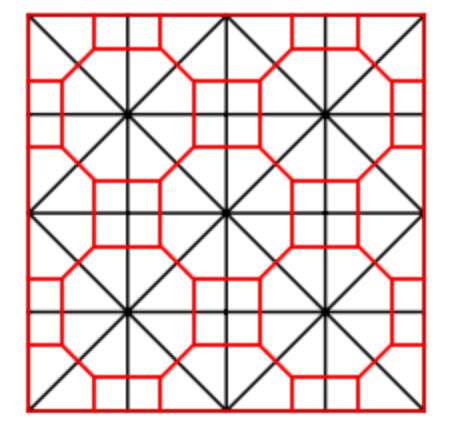
\includegraphics[width=0.5\linewidth]{Materials/ControlVolume}
	\caption{Our mesh drawn in black and our control volumes drawn in red.}
	\label{controlvolume}
\end{figure}

\begin{figure}
	\centering
	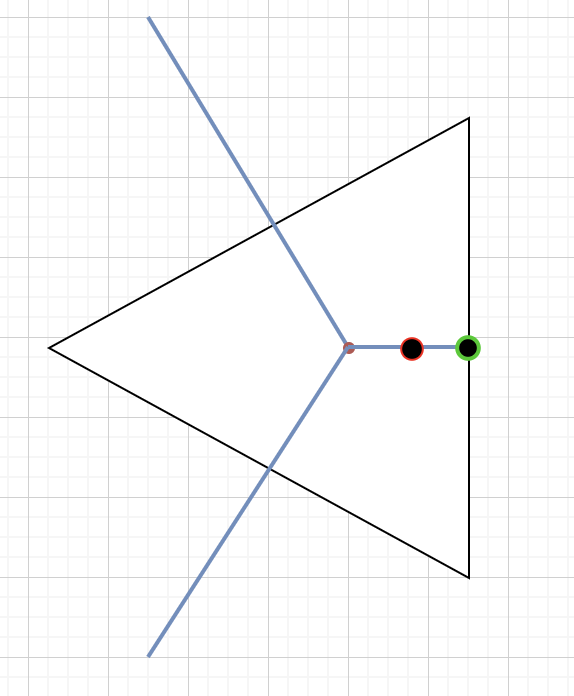
\includegraphics[width=0.5\linewidth]{Materials/boundary}
	\caption{Small error introduced by not using shape functions for interpolation. Blue lines illustrate edges in control volumes and the black lines illustrate a single boundary triangle in our mesh.}
	\label{boundary}
\end{figure}

\subsection{Handling of unit circle}
In this week's assignment when we look at the right hand side integral, $\int_V \nabla \cdot \mathbf{M}(\mathbf{x})dV$, we require the integrand, $\nabla \cdot \mathbf{M}(\mathbf{x})$, to be a continuous real valued function. When we consider a control volume completely outside the unit circle $\mathbf{M}(\mathbf{x})$ is per definition $[0,0]^T$ and thus continuous. When we consider a control volume completely inside the unit circle $\mathbf{M}(\mathbf{x})$ is per definition $[0,-1]^T$ and thus also continuous. However, when we have a control volume which is partially inside and partially outside then $\mathbf{M}(\mathbf{x})$ suddenly jumps from one value to another and is thus discontinuous. We can handle this by splitting the integral into two parts, one over the part of the control volume which is outside the unit circle, and one which is inside and then sum the two parts. That is we would have:
\begin{equation*}
	\int_V \nabla \cdot \mathbf{M}(\mathbf{x})dV = \int_{V_{inside}} \nabla \cdot \mathbf{M}(\mathbf{x})dV + \int_{V_{outside}} \nabla \cdot \mathbf{M}(\mathbf{x})dV
\end{equation*}
This split can either be done on the fly when we realise our control volume is getting split by the unit circle, or we could preemptively design our control volumes such that their boundaries conforms with the unit circle.
\subsection{Difference between Finite Methods}
FVM resembles some of the same concepts as FEM as in both methods we start with a big system which we then divide into smaller subsystems which we then can solve more easily. However, where FEM uses trial functions and integration by parts to convert from strong form to weak form, FVM takes a more direct approach and uses Gauss-Divergence theorem to get surface integrals. FEM also relies on the approximation from using shape functions to interpolate positions inside the domain, where FVM can make use of shape functions, but can also as seen earlier, make use of the outward unit normal from the control volumes. Comparing to FDM, FVM and FEM are much more easily applied to unstructured meshes as it is not always obvious which nodes to use for FDM in an unstructured mesh. However, FDM can quite easily be formally verified though analysis of the Taylor remainder terms, which is not as obviously done for FVM and FEM.